\chapter{基本概念}

信号与系统的概念广泛存在于各个领域。
可以说,当今科技的发展离不开该理论的发展。
信号与系统这门学科就是将各个领域的问题抽象,用数学语言描述和分析,是介于数学和具体学科之间的一门科学。

本章介绍信号和系统的基本概念,并给出几个基本例子。

本章要点:
\begin{itemize}
    \item 信号和系统的概念。
    \item 基本信号:正弦、指数、阶跃、冲激。
    \item 系统的重要特性:线性、时不变、因果。
\end{itemize}

\newpage
\section{信号与系统概述}

本节介绍信号和系统的概念。

本节要点:
\begin{itemize}
    \item 掌握信号、系统及其相关概念。
\end{itemize}

%============================================================
\subsection{信号的概念}

\begin{definition}[信号]
在数学的角度,{\bf 信号}(signal)就是函数,自变量可以是时间、空间等,可以是一元函数,也可以是多元函数。
本书讨论的信号是以时间为自变量的一元函数,通常记为$x\left( t \right) $。
\end{definition}

物理意义上,信号指的是一个物体的状态。
若物体是一实物,则状态可以是物体的位移、速度。
若物体是一场,则状态可以是场强、电压、电流。
总之,信号描述的是一个物体的状态随时间的变化。

可以定义信号的{\bf 能量}和{\bf 功率}:
\begin{align*}
&E=\int_{t_1}^{t_2}{\left| x\left( t \right) \right|^2dt} \\
&P=\frac{1}{t_2-t_1}\int_{t_1}^{t_2}{\left| x\left( t \right) \right|^2dt}
\end{align*}
从能量和功率的角度,信号可以分有限能量信号$E_{\infty}<\infty $、有限功率信号$P_{\infty}<\infty $和能量功率均无限的信号。
而且易得,如果有限能量必然功率为0,如果有限功率必然能量无穷。

这个“功率”和“能量”是纯粹信号与系统上的概念。
虽然和具体物理意义无关,但还是有抽象层面的关系,如弹性势能$E=\frac{1}{2}kl^2$,动能$E=\frac{1}{2}mv^2$。

~

信号与系统中一个重要的概念就是信号的变换,对于以时间为自变量的信号指的就是时间轴的变换:
\begin{itemize}
    \item {\bf 时移}(time shift):$x\left( t-t_0 \right) $,表示信号延迟,或者波形右移。
    \item {\bf 尺变}(time scaling):$x\left( at \right) $,$a>1$表示信号变快,波形压缩,$a<1$表示信号变慢,波形伸长,$a=-1$表示信号{\bf 反转}(time reversal)。
    \item {\bf 周期}:若信号有$x\left( t+T \right) =x\left( t \right) $,则称为{\bf 周期信号}(periodic signal),最小正值$T$称为{\bf 基波周期}(fundamental period)。
    \item {\bf 奇偶性}:若信号有$x\left( t \right) =x\left( -t \right) $,称为{\bf 偶信号}(even),若$x\left( t \right) =-x\left( -t \right) $,称为{\bf 奇信号}(odd),易得,所有信号都可以分解为奇信号和偶信号的和:
    \begin{align*}
    &x_{even}\left( t \right) =\frac{1}{2}\left[ x\left( t \right) +x\left( -t \right) \right] \\
    &x_{odd}\left( t \right) =\frac{1}{2}\left[ x\left( t \right) -x\left( -t \right) \right]
    \end{align*}
\end{itemize}

\begin{tcolorbox}
注,$x\left( t \right) =C$是周期信号,但没有基波周期。
\end{tcolorbox}

%============================================================
\subsection{系统和响应的概念}

\begin{definition}[系统]
{\bf 系统}(system)是组件与端口的互连,通过这些端口可以输出输入信息。
\end{definition}

我们称一组描述输入输出之间相互关系的数学方程为{\bf 系统的数学模型}(mathematical model)。
数学模型是一种描述系统的数学工具,好的数学模型是需要在精确性和简单性之有良好的平衡,两大基本数学模型:
\begin{itemize}
    \item {\bf 输入输出模型}(input/output model):描述输入信号和输出信号之间关系,具体分:
    \begin{itemize}
        \item {\bf 微分方程}(differential equation)和{\bf 差分方程}(difference equation),
        \item {\bf 卷积模型}(convolution model),
        \item {\bf 傅里叶变换}(Fourier transform),
        \item {\bf 传递函数}(transfer function);
    \end{itemize}
    \item {\bf 状态模型}(state model):描述输入、状态、输出之间关系。
\end{itemize}
其中,傅里叶变换可视为传递函数的一个特例。

\begin{definition}[响应]
对于一个特定的输入或系统本身状态,系统会产生一个特定的输出,称为{\bf 响应}(response)。根据引起响应的不同原因,响应可以分为:
\begin{itemize}
    \item {\bf 零输入响应}(zero input):系统响应仅由其初始状态引起,输入始终为0;
    \item {\bf 零状态响应}(zero state):系统初始状态为0,响应仅由输入引发。
\end{itemize}
\end{definition}

\begin{tcolorbox}
为简化讨论,本笔记讨论只有一个输入和一个输出的系统,且系统默认都是零状态响应。
\end{tcolorbox}









\newpage
\section{连续信号}

本节介绍连续信号,并给出4种基本的连续信号。

本节要点:
\begin{itemize}
    \item 掌握连续信号的概念;
    \item 熟悉4个基本连续信号。
\end{itemize}

%============================================================
\subsection{连续信号的概念}

\begin{definition}[连续信号]
当时间变量$t$取值实数时,我们称信号为{\bf 连续信号}(continuous-time signal)或{\bf 模拟信号}(analog signal),通常记为$x\left( t \right) $。
\end{definition}

%============================================================
\subsection{正弦信号}

\[
x\left( t \right) =A\sin \left( \omega t+\varphi \right)
\]
\begin{itemize}
    \item $A$:振幅;
    \item $\omega $:角频;
    \item $\varphi $:相位。
\end{itemize}
周期和频率:
\[
T=\frac{2\pi}{\omega} \qquad f=\frac{1}{T}=\frac{\omega}{2\pi} \qquad \omega =2\pi f
\]

%============================================================
\subsection{指数信号}

\[
x\left( t \right) =Ae^{at}
\]

当$a$为实数,信号的定义域和值域都是实数,称为{\bf 实指数信号}。
当$a>0$时,信号发散,如原子弹爆炸;当$a<0$时,信号衰减;当$a=0$时,信号为常数。
在实际系统中,一般信号都是衰减信号,所以写成:
\[
x\left( t \right) =Ae^{-\frac{t}{\tau}} \qquad \tau >0,t\geqslant 0
\]
其中,$\tau $称为{\bf 时间常数},反映了信号的衰减速度。

\begin{tcolorbox}
曲线$x\left( t \right) =Ae^{-\frac{t}{\tau}}$过曲线上点$\left( t_0,Ae^{-\frac{t_0}{\tau}} \right) $的切线方程:
\[
x\left( t \right) -Ae^{-\frac{t_0}{\tau}}=-\frac{A}{\tau}e^{-\frac{t_0}{\tau}}\left( t-t_0 \right)
\]
交于{\it t}轴:
\begin{align*}
&\because -Ae^{-\frac{t_0}{\tau}}=-\frac{A}{\tau}e^{-\frac{t_0}{\tau}}\left( t-t_0 \right) \\
&\therefore t=t_0+\tau
\end{align*}
这里可以得到衰减的实指数信号的一个特征,曲线切线与{\it t}轴的交点和切点的时间差永远是$\tau $。
\end{tcolorbox}

当$a$为复数$s=\sigma +i\omega $时信号为:
\[
x\left( t \right) =Ae^{st}
\]
此时信号的值域都是复数,称为{\bf 复指数信号},模、实部和虚部如下:
\begin{align*}
&\left| x\left( t \right) \right|=Ae^{\sigma t} \\
&\mathrm{Re}\left[ x\left( t \right) \right] =Ae^{\sigma t}\mathrm{Re}\left[ e^{i\omega t} \right] =Ae^{\sigma t}\cdot \cos \left( \omega t \right) \\
&\mathrm{Im}\left[ x\left( t \right) \right] =Ae^{\sigma t}\mathrm{Im}\left[ e^{i\omega t} \right] =Ae^{\sigma t}\cdot \sin \left( \omega t \right)
\end{align*}
实部和虚部都是正弦信号,且$T=2\pi /\omega $,两者“对称”振荡,整体由指数包络。
$\sigma $决定发散还是衰减,系统能量:
\[
E_{\infty}=\int_0^{+\infty}{\left| Ae^{st} \right|^2dt}=A^2\int_0^{+\infty}{e^{2\sigma t}dt}=\frac{A^2}{2\sigma}\left( \left. e^{2\sigma t} \right|_{0}^{+\infty} \right)
\]
当时$\sigma <0$,信号是有限能量。

物理中,复指数较实指数更为普遍。复指数代表着两个状态或者两种能量的相互转化,如弹簧的简谐振动、RC振荡电路。
$\omega $决定了转化速度,$\sigma $决定了系统是否对外辐射能量。
所以在复指数中,一个变量$s=\sigma +i\omega $就表示了系统的内在运动和对外关系。

当$s$为纯虚数时,写为:
\[
x\left( t \right) =Ae^{i\omega t}=A\left( \cos \omega t+i\sin \omega t \right)
\]
称为{\bf 纯虚指数信号}。
只有当$s$为纯虚数时,信号才是周期信号。
纯虚指数信号另一个特征是有限功率:
\[
P_{\infty}=\underset{T\rightarrow \infty}\lim \frac{1}{T}\int_{-\frac{T}{2}}^{\frac{T}{2}}{\left| Ae^{i\omega t} \right|^2dt}=\underset{T\rightarrow \infty}\lim \frac{1}{T}\int_{-\frac{T}{2}}^{\frac{T}{2}}{A^2dt}=A^2
\]

如果一个信号是纯虚指数信号,表示系统对外没有能量交换,如无阻尼谐振子。

%============================================================
\subsection{单位阶跃和单位冲激}

\begin{figure}[h]
\centering
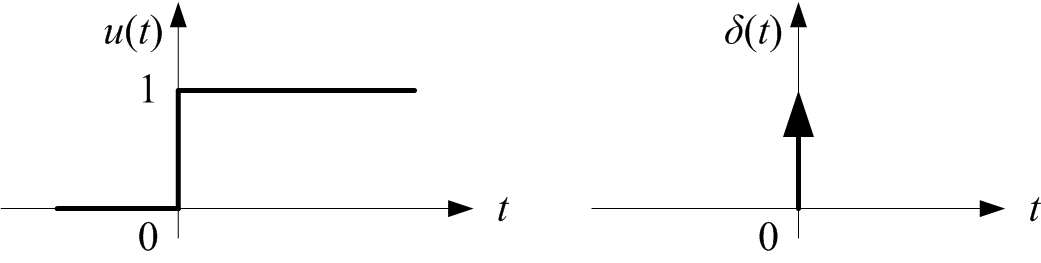
\includegraphics[height=2cm]{1.2.4-1.png}
\end{figure}
\[
u\left( t \right) =\begin{cases}
	1 \quad t\geqslant 0\\
	0 \quad t<0\\
\end{cases} \qquad \begin{array}{l}
	\delta \left( t \right) =0 \quad t\ne 0\\
	\int_{-\infty}^{+\infty}{\delta \left( \tau \right) d\tau}=1\\
\end{array}
\]
两者关系:
\[
\begin{cases}
	u\left( t \right) =\int_{-\infty}^t{\delta \left( \tau \right) d\tau}\\
	\delta \left( t \right) =\frac{du\left( t \right)}{dt}\\
\end{cases}
\]
严格来讲,因为$u\left( t \right) $在$t=0$不连续,所以$\delta \left( t \right) $不是$t=0$的导数。
但不妨碍讨论。

从$u\left( t \right) =\int_{-\infty}^t{\delta \left( \tau \right) d\tau}$来看,$u\left( t \right) $是$\delta \left( t \right) $的积分上限函数,即是积分区间的移动。
令$\tau =t-\sigma $,有:
\begin{align*}
&d\tau =d\left( t-\sigma \right) =-d\sigma \\
&u\left( t \right) =\int_{-\infty}^t{\delta \left( \tau \right) d\tau}=-\int_0^{+\infty}{\delta \left( t-\sigma \right) d\sigma}
\end{align*}
可以认为积分区间不动,$u\left( t \right) $是$\delta \left( t \right) $的移动的结果。
\begin{figure}[h]
\centering
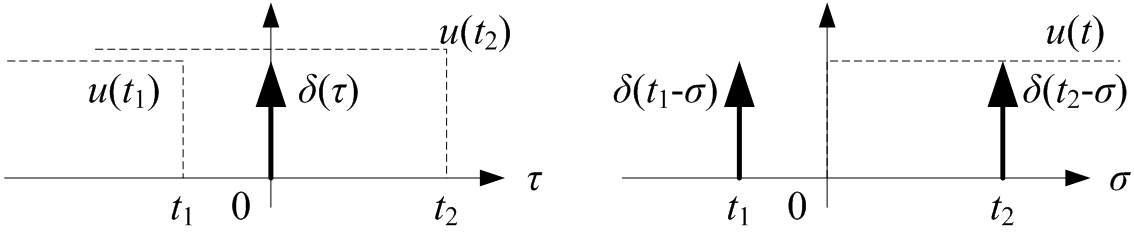
\includegraphics[height=2cm]{1.2.4-2.png}
\end{figure}

$\delta \left( t \right) $的特征:
\begin{itemize}
    \item 偶函数,$\delta \left( t \right) =\delta \left( -t \right) $。
    \item 单位面积,$\int_{-\infty}^{+\infty}{\delta \left( \tau \right) d\tau}=1$,也即能量有限。
    \item 尺度变换性质,$\delta \left( at \right) =\frac{1}{\left| a \right|}\delta \left( t \right) $。
    \item 筛选性,$f\left( t \right) =\int_{-\infty}^{+\infty}{f\left( t \right) \delta \left( \tau -t \right) d\tau}$。
\end{itemize}

$\delta \left( t \right) $的导数:将两个“微小错开”的正负单位冲激的叠加称为{\bf 单位冲激偶},记为$\delta '\left( t \right) $,有如下特征:
\begin{itemize}
    \item 奇函数,$\delta '\left( t \right) =-\delta '\left( -t \right) $。
    \item 面积为0,$\int_{-\infty}^{+\infty}{\delta '\left( \tau \right) d\tau}=0$,也即无能量。
    \item 筛选性,$\int_{-\infty}^{+\infty}{f\left( t \right) \delta '\left( \tau -t \right) d\tau}=-f'\left( t \right) $。
\end{itemize}

%============================================================
\subsection{广义导数}

\begin{definition}[广义导数]
假设信号$x\left( t \right) $在$t_0$不可导,我们定义$x\left( t \right) $在$t_0$的{\bf 广义导数}(generalized derivative)为:
\[
\left. \frac{dx\left( t \right)}{dt} \right|_{t=t_0}=\left[ x\left( {t_0}^+ \right) -x\left( {t_0}^- \right) \right] \delta \left( t-t_0 \right)
\]
即用冲激函数筛选$\left[ x\left( {t_0}^+ \right) -x\left( {t_0}^- \right) \right] \delta \left( t-t_0 \right) $代替$t_0$处的导数。
\end{definition}






\newpage
\section{离散信号}

本节介绍离散信号,并给出2种基本的离散信号。

本节要点:
\begin{itemize}
    \item 掌握离散信号的概念;
    \item 熟悉2个基本离散信号。
\end{itemize}

%============================================================
\subsection{离散信号的概念}

\begin{definition}[离散信号]
当时间变量取离散值$t=t_n,n=0,\pm 0,\pm 2,\cdots $时,我们称信号为{\bf 离散信号}(discrete-time signal),记为$x\left[ n \right] $,其中$n$表示$t_n$,即第$n$个时间采样点。
一般我们通过对连续信号的周期性采样获得离散信号,即:
\begin{align*}
&n=\frac{t}{T} \\
&x\left[ n \right] =\left. x\left( t \right) \right|_{t=nT}=x\left( nT \right)
\end{align*}
其中,$T$为采样周期,单位s。
\end{definition}

虽然不硬性规定$t_n$之间的间隔,但一般我们还是等间隔处理,即“周期性”采样。

%============================================================
\subsection{单位阶跃和单位冲激}

\begin{figure}[h]
\centering
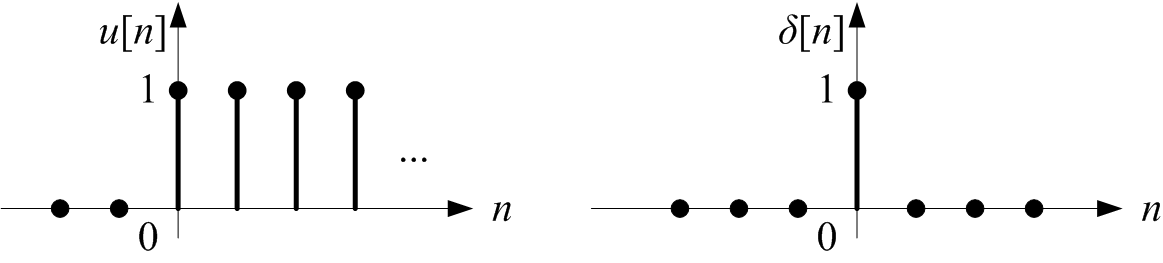
\includegraphics[height=2cm]{1.3.2-1.png}
\end{figure}
\[
u\left[ n \right] =\begin{cases}
	1 \quad n=0,1,2,\cdots\\
	0 \quad n=-1,-2,\cdots\\
\end{cases} \quad \delta \left[ n \right] =\begin{cases}
	1 \quad n=0\\
	0 \quad n=\pm 1,\pm 2,\cdots\\
\end{cases}
\]






\newpage
\section{系统的特性}

本节介绍系统的4大特性。

本节要点:
\begin{itemize}
    \item 掌握系统的4大特性:线性性,时不变,因果性,有限维度。
\end{itemize}

\begin{tcolorbox}
本书讨论的系统,都符合这4大特性。
\end{tcolorbox}

%============================================================
\subsection{线性和时不变}

若系统满足:
\begin{itemize}
    \item $x_1\left( t \right) +x_2\left( t \right) \rightarrow y_1\left( t \right) +y_2\left( t \right) $:称为{\bf 可加的}(additive),
    \item $ax\left( t \right) \rightarrow ay\left( t \right) $:称为{\bf 均匀的},或{\bf 齐次的}(homogeneous)。
\end{itemize}
若都满足,称为{\bf 线性的}(linear)。
严格来讲,讨论线性时,对系统的要求是无初始状态,即零状态。
若系统满足$x\left( t-t_0 \right) \rightarrow y\left( t-t_0 \right) $,称为{\bf 时不变}(time invariant)。
时不变表示系统的特性不随时间变化而变化,如RC电路,短时间看是一个时不变系统。
但长时间看,由于电容电解液的消耗导致电容值发生改变,是一个时变系统。

线性和时不变是系统最重要的两个特性。
如果系统满足线性和时不变,则称为{\bf LTI系统},这样的系统在计算上可以大大简化。
绝大多数自然界系统也都可以认为是LTI系统。
信号与系统这门学科着重研究的就是LTI系统的表述和分析,如何将一个系统建模成LTI,即便无法建模成LTI,那如何近似成一个LTI。

%============================================================
\subsection{记忆和因果}

若输出只与该时刻和之前的输入有关,称系统为{\bf 因果系统}(casual system)。
若系统的输出只取决于当刻的输入,则称为{\bf 无记忆系统}(memoryless system),如电阻,反之,称为{\bf 有记忆系统}(system with memory),如电容。
实际系统中,记忆是直接和能量相联系的,比如电容存储的电荷,车辆保有的动能。
无记忆系统都是因果系统。

能量在系统内部会有某种“惯性”,使得信号在系统内部造成“回响”效果,系统的输出就是之前各个时间点的回响的“混响”效应:
\[
y\left[ n \right] =\sum_{i=-\infty}^n{a_ix\left[ i \right]}=a_nx\left[ n \right] +\sum_{i=-\infty}^{n-1}{a_ix\left[ i \right]}=a_nx\left[ n \right] +y\left[ n-1 \right]
\]
这就是差分(同理也是微分)的由来。
时域模型就是研究系统的回响和混响。

%============================================================
\subsection{有限维度}

若系统的输入输出关系可以用微分方程
\[
y^{\left( n \right)}\left( t \right) = f\left[ y\left( t \right) ,y'\left( t \right) ,\cdots ,y^{\left( n-1 \right)}\left( t \right) , x\left( t \right) ,x'\left( t \right) ,\cdots ,x^{\left( m \right)}\left( t \right) ,t \right]
\]
描述,则称为{\bf 有限维度系统}(finite dimensional system),$n$为系统的{\bf 维度}(dimension)或{\bf 阶}(order)。
特别地,当有限维度系统可以描述为
\[
y^{\left( n \right)}\left( t \right) +\sum_{i=0}^{n-1}{a_i\left( t \right) y^{\left( i \right)}\left( t \right)}=\sum_{i=0}^m{b_i\left( t \right) x^{\left( i \right)}\left( t \right)}
\]
即为{\bf 线性系统}。
若更进一步,当输入输出的系数为常数,即
\[
y^{\left( n \right)}\left( t \right) +\sum_{i=0}^{n-1}{A_iy^{\left( i \right)}\left( t \right)}=\sum_{i=0}^m{B_ix^{\left( i \right)}\left( t \right)}
\]
时,为{\bf 线性时不变系统}。

对于离散系统,若输入输出满足差分方程
\[
y\left[ n \right] = f\left( y\left[ n-1 \right] ,\cdots ,y\left[ n-N \right] ,x\left[ n \right] ,x\left[ n-1 \right] ,\cdots ,x\left[ n-M \right] ,n \right)
\]
称为{\bf 有限维度系统}(finite dimensional system),同样地,$N$称为系统的{\bf 维度}(dimension)或{\bf 阶}(order)。

%============================================================
\subsection{其他特性}

系统的其他特性还包括{\bf 可逆性}。
如编码系统,必须是可逆的,必有且仅有一个与之对应的逆系统进行解码。
如果系统在一个有限的输入下,响应收敛,称为{\bf 稳定的}。
一般来讲稳定性是由于能量消耗的原因。






\newpage
\section{例}

本节以4个实例介绍系统的概念,并给出其时域模型。

%============================================================
\subsection{RC电路}

\begin{example}
如下RC电路,假设电压源为系统输入信号$x\left( t \right) $,电容两端电压看作系统输出信号$y\left( t \right) $,试写出输入输出的微分方程。
\end{example}

\begin{figure}[h]
\centering
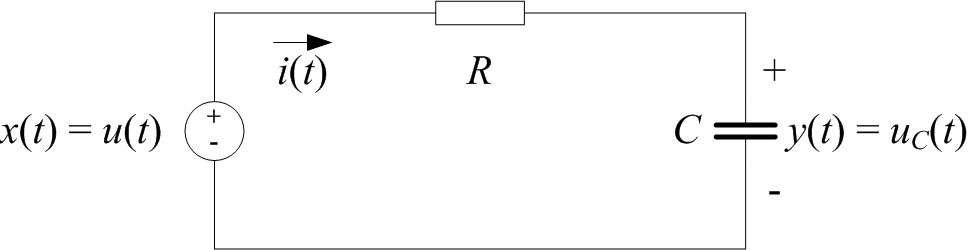
\includegraphics[height=2cm]{1.5.1-1.png}
\end{figure}

根据KVL推导RC电路的输入输出模型:
\begin{align*}
&\because u_C+u_R=u \\
&\therefore y+C\frac{dy}{dt}\cdot R=x \\
&\therefore \frac{dy}{dt}+\frac{1}{RC}y=\frac{1}{RC}x
\end{align*}
只要确定了输入信号$x=u\left( t \right) $,就可通过求解微分方程得到输出信号$y=u_C\left( t \right) $。

\begin{tcolorbox}
该RC电路会在之后的章节中反复讨论。
\end{tcolorbox}

%============================================================
\subsection{汽车运行}

\begin{example}
假设车辆在不光滑路面沿直线行驶,整个车辆作为系统,将发动机的动力视为系统输入$x$,行驶距离视为输出$y$,试写出系统的输入输出的微分方程。
\end{example}

根据牛顿定律我们可以得到车辆的加速度和受力的关系式:
\[
F=Ma
\]
车辆受力除了发动机的输出力之外,还有地面的摩擦力,摩擦力和速度成正比$K$,反向于速度方向,于是:
\[
x-K\frac{dy}{dt}=M\frac{d^2y}{dt^2}
\]
该微分方程即为车辆系统的微分方程。

%============================================================
\subsection{弹簧减震系统}

\begin{example}
如下图,系统由压块(质量$M$)、弹簧(胡克系数$K$)和阻尼器(阻尼系数$D$)组成,将压块受到的外力视为输入$x=F\left( t \right) $,压块位移视为输出$y=S\left( t \right) $,试写出输入输出的微分方程。
\end{example}

\begin{figure}[h]
\centering
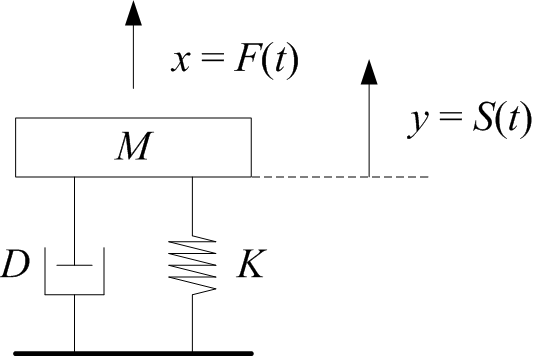
\includegraphics[height=3cm]{1.5.3-1.png}
\end{figure}

依然根据牛顿定律,考察压块的加速度和受力,弹簧施加反向作用力(大小和压块位移成正比),阻尼器施加反向作用力(大小和压块速度成正比),有:
\[
x-D\frac{dy}{dt}-Ky=M\frac{d^2y}{dt^2}
\]

%============================================================
\subsection{钟摆}

\begin{example}
假设有钟摆,输入为小球受的切向于运动方向的力$x=F\left( t \right) $,输出为偏转角$y=\theta \left( t \right) $,试写出输入输出的微分方程。
\end{example}

\begin{figure}[h]
\centering
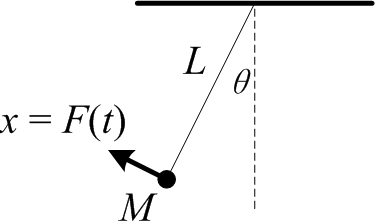
\includegraphics[height=2cm]{1.5.4-1.png}
\end{figure}

小球转动惯量为$I=ML^2$,收到两个外力$x=F\left( t \right) $和重力,它们产生的力矩分别为$xL,MgL\sin y$,根据牛顿定律对转动角加速度和力矩的关系,有:
\[
ML^2\cdot \frac{d^2y}{dt^2}=xL-MgL\sin y
\]
根据这个输入输出模型的描述,系统不是一个线性系统,无法得到解析解。
但是如果考虑偏转角很小$\sin \theta =\theta $有:
\[
ML\cdot \frac{d^2y}{dt^2}=x-Mg\cdot y
\]
变成了线性系统。
通过这样的处理后的系统称为{\bf 小信号系统}(small-signal system)。

\begin{tcolorbox}
有的时候,严格来讲,碰到的系统并不是LTI。
但是考虑到输入输出信号很小的情况下,可以近似用线性模型描述,这样的模型称为该系统的小信号模型。
在一定程度下,可以用一个简单的微分方程代替一个复杂的微分方程来考察系统。
\end{tcolorbox}






\newpage
\section{本章小结}

本章初步定义了一些信号与系统的概念,并举了几个例子。
这些例子涵盖不同的学科,但它们有一个共同的特点,一个输入量通过一个系统的作用产生一个输出量。

\begin{figure}[h]
\centering
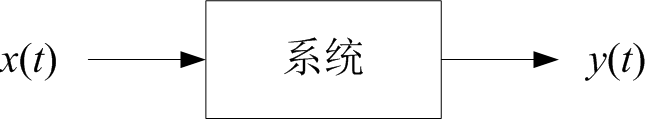
\includegraphics[height=1cm]{1.6-1.png}
\end{figure}

RC电路例子需要特别注意,在今后章节会反复引用。
\begin{figure}[h]
\centering
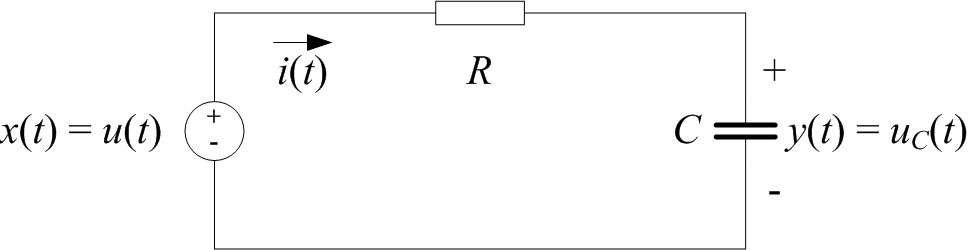
\includegraphics[height=2cm]{1.5.1-1.png}
\end{figure}
\[
\frac{dy}{dt}+\frac{1}{RC}y=\frac{1}{RC}x
\]









